\documentclass{beamer}
\mode<presentation>
{
  \usetheme{Warsaw}      % or try Darmstadt, Madrid, Warsaw, ...
  \usecolortheme{beaver} % or try albatross, beaver, crane, ...
  \usefonttheme{default}  % or try serif, structurebold, ...
  \setbeamertemplate{navigation symbols}{}
  \setbeamertemplate{caption}[numbered]
  \setbeamertemplate{footline}[frame number]
}


\usepackage[english]{babel}
\usepackage[utf8]{inputenc}
\usepackage{graphicx}
\usepackage{pgfpages}

\usepackage{algorithm}
\usepackage[noend]{algorithmic}

\title {PA-EDF}
\subtitle {Preemption-aware algorithm dominating EDF}
\author{Thomas Chapeaux \inst{1}}
\institute[shortinst]{\inst{1} Université Libre de Bruxelles}
\date{Summer 2013}

\begin{document}

\maketitle{}

\begin{frame}{Outline}
    \tableofcontents
\end{frame}

\section{Preemption Model}

\begin{frame}{Model}
    \begin{itemize}
        \item System: set of tasks $\tau_i = (O_i, C_i, D_i, T_i, \alpha_i)$
        \item $\alpha_i$: per-task preemption cost
        \item Preemption jobs must go through a \textbf{preemption recovery period (PRP)} of size $\alpha_i$ upon re-entering the system.
        \item The preemption recovery period is non-interruptible.
    \end{itemize}
    \begin{columns}[c]
    \column{0.4\textwidth}
        \begin{center}
            \begin{tabular}{|r|c|c|c|c|c|}
                \hline
                            & $O_i$ & $C_i$ & $D_i$ & $T_i$ & $\alpha_i$ \\ \hline
                $\tau_1$    & 0     & 5     & 11    & 11    & 2     \\ \hline
                $\tau_2$    & 4     & 1     & 1     & 11    & 2     \\ \hline
                $\tau_2$    & 6     & 1     & 2     & 11    & 2     \\ \hline
            \end{tabular}
        \end{center}
    \column{0.6\textwidth}
        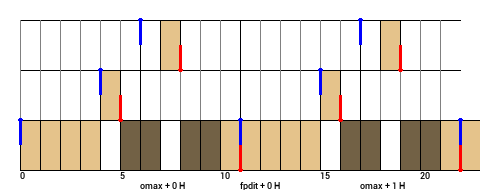
\includegraphics[width=1.1\textwidth]{figs/atomicpreemption_example.png}
    \end{columns}
\end{frame}

\section{Properties of costly-preemption systems}

\begin{frame}{Outline}
    \tableofcontents[currentsection]
\end{frame}


\subsection{Non-optimality of EDF}

\begin{frame}{Non-optimality of EDF}
    EDF is non-optimal. Example:

    \begin{columns}[c]
    \column{0.5\textwidth}
        \begin{center}
            \begin{tabular}{|r|c|c|c|c|c|}
                \hline
                            & $O_i$ & $C_i$ & $D_i$ & $T_i$ & $\alpha_i$ \\ \hline
                $\tau_1$    & 1     & 2     & 4     & 4     & 2     \\ \hline
                $\tau_2$    & 0     & 3     & 6     & 6     & 2     \\ \hline
            \end{tabular}
        \end{center}
        Other anomalies of EDF scheduling:
        \begin{itemize}
            \item The system can stabilize after $O_{max} + 2H$
            \item A deadline miss can occur before stabilization then never again. (?)
        \end{itemize}
    \column{0.5\textwidth}
        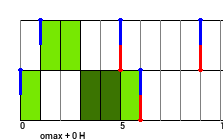
\includegraphics[width=0.9\textwidth]{figs/edfNonOptimal_EDF.png}

        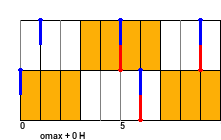
\includegraphics[width=0.9\textwidth]{figs/edfNonOptimal_PALLF.png}
    \end{columns}

    LLF is also non-optimal.
\end{frame}

\subsection{Other properties}

\begin{frame}{Other properties}
    As we saw previously, an optimal algorithm for constrained-deadline monoprocessor systems with preemption costs has to be :
    \begin{itemize}
        \item Dynamic (jobs priority must be able to change online)
        \item Claivoyant (jobs arrival time must be known)
        \item Idling (Even with active jobs in the system)
        \item Minimizing preemptions
    \end{itemize}
    % An optimal algorithm has to be dynamic
    % \begin{columns}[c]
    % \column{0.5\textwidth}
    %     \begin{center}
    %         \begin{tabular}{|r|c|c|c|c|c|}
    %             \hline
    %                         & $O_i$ & $C_i$ & $D_i$ & $T_i$ & $\alpha_i$ \\ \hline
    %             $\tau_1$    & 5     & 1     & 1     & 8     & 1     \\ \hline
    %             $\tau_2$    & 3     & 1     & 1     & 8     & 1     \\ \hline
    %             $\tau_3$    & 0     & 1     & 5     & 8     & 1     \\ \hline
    %             $\tau_4$    & 0     & 4     & 8     & 8     & 1     \\ \hline
    %         \end{tabular}
    %     \end{center}
    % \column{0.5\textwidth}
    %     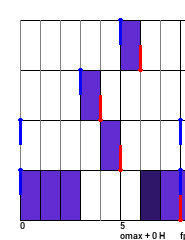
\includegraphics[width=0.8\textwidth]{figs/dponly_palff.png}
    % \end{columns}

\end{frame}

% \subsection{Idling scheduler}

% \begin{frame}{Idling scheduler}
%     An optimal algorithm has to be idling.

%     \begin{columns}[c]
%     \column{0.5\textwidth}
%         \begin{center}
%             \begin{tabular}{|r|c|c|c|c|c|}
%                 \hline
%                             & $O_i$ & $C_i$ & $D_i$ & $T_i$ & $\alpha_i$ \\ \hline
%                 $\tau_1$    & 1     & 1     & 1     & 8     & 9     \\ \hline
%                 $\tau_2$    & 0     & 3     & 5     & 8     & 9     \\ \hline
%                 $\tau_3$    & 0     & 3     & 8     & 8     & 9     \\ \hline
%             \end{tabular}
%         \end{center}
%     \column{0.5\textwidth}
%         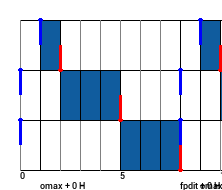
\includegraphics[width=\textwidth]{figs/mustIdle_PALLF.png}
%     \end{columns}
% \end{frame}

\begin{frame}{When to idle?}
    \begin{block}{Definition}
        The \textbf{earliest preemptive arrival ($epa$)} of a job is the earliest arrival of another job with higher priority.
    \end{block}

    \begin{block}{Definition}
        The \textbf{minimal termination time ($mtt$)} of a job is the instant at which the job will end if it begins executing immediately until completion.
    \end{block}

    A job $j$ should \textbf{NOT} execute at instant $t$ iff:
    \begin{itemize}
        \item The job was not executing at $t-1$
        \item It will certainly be preempted ($epa(j) < mtt(j)$)
        \item It will be preempted in less than $\alpha_i$ units ($epa(j) - t < \alpha_i$)
    \end{itemize}
\end{frame}

% \subsection{Limited preemption}

% \begin{frame}{Preemptions should be avoided}
%     \begin{itemize}
%         \item Each preemption adds $\alpha_i$ to the system load
%         \item $\Rightarrow$ Only use preemption if absolutely necessary
%         \item A job $j_1$ arriving at time $t$ while $j_2$ is executing
%         \begin{itemize}
%             \item must be preemptive if its laxity ($\ell(t, j_1) = D_1 - C_1$) is smaller than the remaining computation time of $j_2$.
%         \end{itemize}
%         \item Otherwise $\rightarrow$ ? (Choose job with less laxity?)
%     \end{itemize}

%     \begin{center}
%         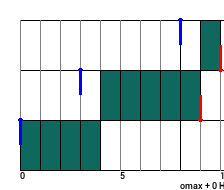
\includegraphics[width=0.3\textwidth]{figs/HardPreemChoice_NoPreempt.png}
%         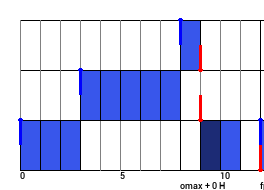
\includegraphics[width=0.35\textwidth]{figs/HardPreemChoice_CKEDF.png}
%     \end{center}
% \end{frame}

\section{Our algorithm: PA-EDF}

\begin{frame}{Outline}
    \tableofcontents[currentsection]
\end{frame}

\subsection{Algorithm}

\begin{frame}{Algorithm (I)}
\begin{algorithm}[H]
    \begin{algorithmic}[1]
        \IF{$t$ is an idle instant}
            \IF{$j$ would be preempted at $t + \alpha_j$ (see Algo.~\ref{alg:preemp})}
                \RETURN $- \infty$
            \ELSE
                \RETURN $1 / j.deadline$
            \ENDIF
        \ELSIF{$j$ is a busy job}
            \IF {$j$ must be preempted now (see Algo.~\ref{alg:preemp})}
                \RETURN $- \infty$
            \ELSE
                \RETURN 1
            \ENDIF
        \ENDIF
        \RETURN $1 / j.deadline$
    \end{algorithmic}
        \caption{Priority of job $j$ at time $t$ with PA-EDF}
        \label{alg:prio}
    \end{algorithm}
    \begin{itemize}
        \item Complexity: $O($Complexity of Algo.~\ref{alg:preemp})$)$
    \end{itemize}
\end{frame}

\begin{frame}{Algorithm (II)}
\begin{algorithm}[H]
    \begin{algorithmic}[1]
    \STATE cumulCompLeft $\leftarrow$ compLeft(j)
    \FORALL {active jobs $j'$ s.t. $j'.deadline \leqslant j.deadline$}
        \IF {$j'$ was preempted}
            \STATE lax $\leftarrow j'.deadline - t - j'.compLeft$ - $\alpha_j'$
        \ELSE
            \STATE lax $\leftarrow j'.deadline - t - j'.compLeft$
        \ENDIF
        \IF {lax $<$ cumulCompLeft}
            \RETURN True
        \ELSE
            \STATE cumulCompLeft += $j'.compLeft$
        \ENDIF
    \ENDFOR
    \RETURN False
    \end{algorithmic}
        \caption{Should job $j$ be preempted at time $t$?}
        \label{alg:preemp}
    \end{algorithm}
    \begin{itemize}
        \item Complexity: for constrained deadline (at most 1 job per task): $O(n)$
    \end{itemize}
\end{frame}

\subsection{Example}

\begin{frame}{Example}

        \begin{center}
            \begin{tabular}{|r|c|c|c|c|c|}
                \hline
                            & $O_i$ & $C_i$ & $D_i$ & $T_i$ & $\alpha_i$ \\ \hline
                $\tau_1$    & 0     & 1     & 12    & 12    & 2     \\ \hline
                $\tau_2$    & 2     & 3     & 20    & 20    & 2     \\ \hline
                $\tau_3$    & 0     & 26    & 45    & 45    & 2     \\ \hline
            \end{tabular}
        \end{center}

        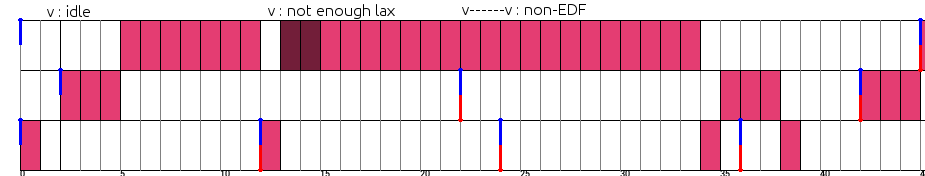
\includegraphics[width=1\textwidth]{figs/PAEDF_example.png}

\end{frame}

\subsection{Dominance over EDF}

\begin{frame}{Dominance over EDF}
    \begin{center}
        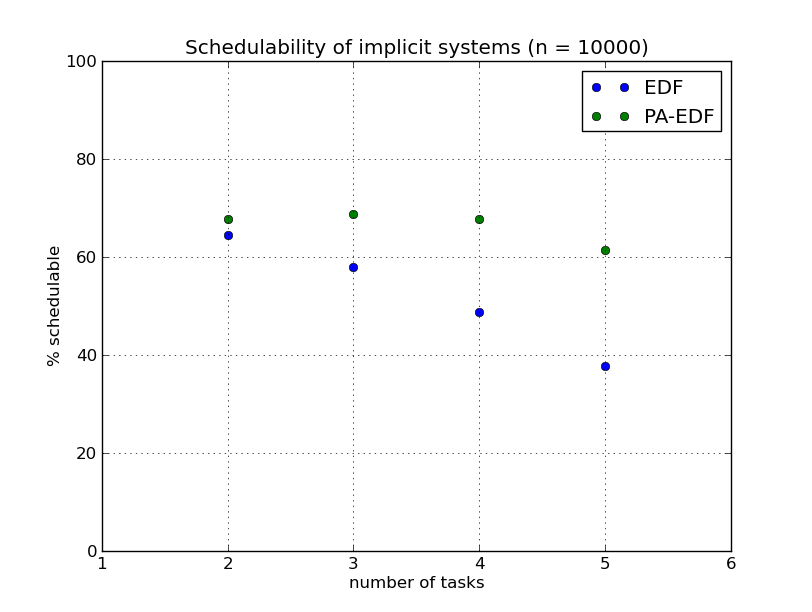
\includegraphics[width=0.65\textwidth]{figs/ptedf_dominance.png}
    \end{center}
    \begin{itemize}
        \item Implicit systems, $\alpha_i = 2 \; \forall i$.
        \item No EDF-schedulable system was not PA-EDF-schedulable.
        \item Optimality of PA-EDF? (for implicit systems)
    \end{itemize}
\end{frame}

\section{Bibliography}


\end{document}
